\documentclass[11pt,a4paper]{article}

% Pacotes essenciais de formatação e codificação
\usepackage[utf8]{inputenc}
\usepackage[T1]{fontenc}
\usepackage[brazilian]{babel}
\usepackage{geometry}
\geometry{top=2.2cm, bottom=2.2cm, left=2.2cm, right=2.2cm}
\usepackage{amsmath,amssymb}
\usepackage{graphicx}
\usepackage{xcolor}
\usepackage{hyperref}
\usepackage{fancyhdr}
\usepackage{booktabs}
\usepackage{enumitem}
\usepackage{tcolorbox}
\tcbuselibrary{skins,breakable}

% Definição da Paleta de Cores Oficial do RosiView
\definecolor{rosiblue}{HTML}{0284C7}
\definecolor{rosidark}{HTML}{0F172A}
\definecolor{rosilight}{HTML}{F8FAFC}
\definecolor{rosigray}{HTML}{334155}
\definecolor{rosigreen}{HTML}{10B981}
\definecolor{rosiamber}{HTML}{D97706}
\definecolor{rosired}{HTML}{EF4444}
\definecolor{boxbg}{HTML}{F1F5F9}

% Configuração de Links e Metadados do PDF
\hypersetup{
    colorlinks=true,
    linkcolor=rosiblue,
    citecolor=rosiblue,
    urlcolor=rosiblue,
    pdftitle={Manual do Usuário - RosiView v0.3},
    pdfauthor={Profª Rosiane Ribeiro Rocha - IFES},
    pdfsubject={Técnico em Mecatrônica - Sistemas de Controle}
}

% Configuração de Cabeçalho e Rodapé das páginas de conteúdo
\pagestyle{fancy}
\fancyhf{}
\lhead{\small\textcolor{rosigray}{\textbf{RosiView v0.3} --- Manual do Usuário}}
\rhead{\small\textcolor{rosigray}{IFES --- Técnico em Mecatrônica --- Sistemas de Controle}}
\cfoot{\small\thepage}
\renewcommand{\headrulewidth}{0.6pt}
\renewcommand{\footrulewidth}{0.4pt}

% Estilo de Caixas Informativas (TColorBox)
\newtcolorbox{dica}[1][]{
    enhanced,
    colback=boxbg,
    colframe=rosiblue,
    fonttitle=\bfseries,
    title=Dica Prática,
    arc=3mm,
    boxrule=1pt,
    left=4mm, right=4mm, top=3mm, bottom=3mm,
    #1
}

\newtcolorbox{atencao}[1][]{
    enhanced,
    colback=rosilight,
    colframe=rosiamber,
    fonttitle=\bfseries,
    title=Observação Importante,
    arc=3mm,
    boxrule=1.2pt,
    left=4mm, right=4mm, top=3mm, bottom=3mm,
    #1
}

\newtcolorbox{destaque}[1][]{
    enhanced,
    colback=rosilight,
    colframe=rosigreen,
    fonttitle=\bfseries,
    title=Destaque Tecnológico,
    arc=3mm,
    boxrule=1pt,
    left=4mm, right=4mm, top=3mm, bottom=3mm,
    #1
}

\begin{document}

% ==============================================================================
% PÁGINA 1: CAPA OFICIAL
% ==============================================================================
\begin{titlepage}
    \centering
    \vspace*{0.6cm}

    {\large \textbf{INSTITUTO FEDERAL DO ESPÍRITO SANTO --- CAMPUS SERRA}}\\[0.3cm]
    {\normalsize \textbf{TÉCNICO EM MECATRÔNICA INTEGRADO AO ENSINO MÉDIO}}\\[0.3cm]
    {\normalsize \textbf{SISTEMAS DE CONTROLE}}\\[1.5cm]

    % Arte do ícone grande da aplicação
    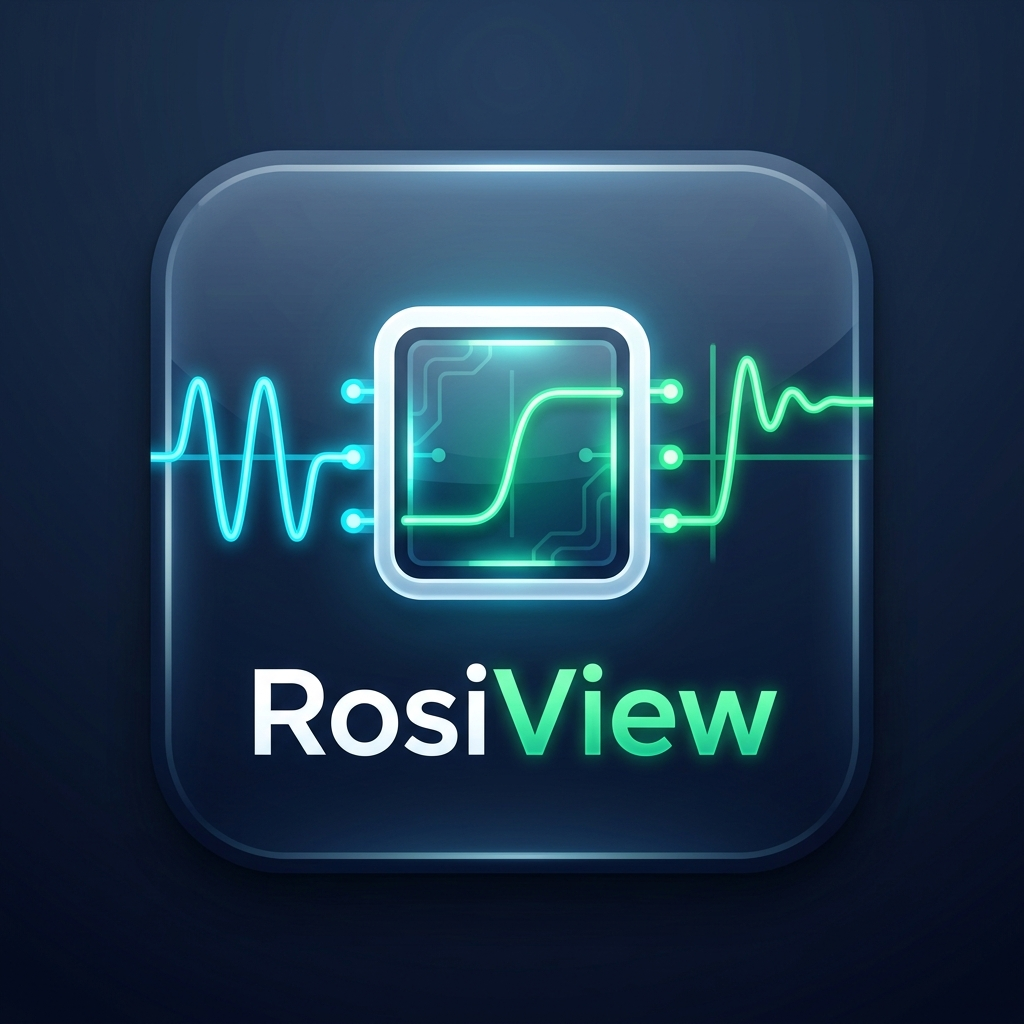
\includegraphics[width=5.8cm]{rosiview_icon.png}\\[1.0cm]

    {\LARGE \bfseries \textcolor{rosiblue}{Ambiente de Instrumentação Virtual}}\\[0.25cm]
    {\LARGE \bfseries \textcolor{rosiblue}{e Programação por Fluxo de Dados}}\\[1.6cm]

    {\huge \bfseries Manual do Usuário --- Versão v0.3}\\[1.8cm]

    \vfill

    \begin{tcolorbox}[colback=rosilight,colframe=rosiblue,arc=3.5mm,width=0.88\textwidth,center,halign=center]
        \vspace{0.25cm}
        {\normalsize \textbf{Desenvolvido por:} Prof\textsuperscript{a} Rosiane Ribeiro Rocha}\\[0.25cm]
        {\normalsize \textbf{Versão da Plataforma:} v0.3 (Distribuição Acadêmica Multiplataforma)}\\[0.25cm]
        {\normalsize \textbf{Ano Letivo:} 2026}
        \vspace{0.25cm}
    \end{tcolorbox}

    \vspace*{0.6cm}
\end{titlepage}

% ==============================================================================
% PÁGINA 2: EXCLUSIVA PARA O SUMÁRIO
% ==============================================================================
\clearpage
\setcounter{page}{2}
\thispagestyle{fancy}
\vspace*{0.5cm}
\tableofcontents
\clearpage

% ==============================================================================
% SEÇÃO 1: INTRODUÇÃO
% ==============================================================================
\section{Introdução ao RosiView}

O \textbf{RosiView} é um ambiente computacional moderno de instrumentação virtual desenvolvido para o ensino e prática de sistemas de controle, mecatrônica e aquisição de dados no IFES. Inspirado na arquitetura clássica do consagrado software LabVIEW$^\circledR$, o RosiView adota o paradigma de \textbf{programação por fluxo de dados} (\textit{dataflow programming}).

Diferente de linguagens baseadas em texto procedimental (como C ou Python puro), no RosiView os programas são construídos conectando blocos funcionais através de cabos virtuais (\textit{wires}). Um bloco executa estritamente quando todos os dados em seus terminais de entrada tornam-se disponíveis, garantindo concorrência natural e grande expressividade visual.

\subsection{As Duas Visões Complementares}
Todo projeto no RosiView é constituído por duas partes integradas:
\begin{enumerate}[leftmargin=*]
    \item \textbf{Painel Frontal (IHM --- Interface Homem-Máquina):} É a tela de controle do operador. Aqui ficam os botões giratórios (\textit{knobs}), seletores de nível (\textit{sliders}), interruptores, telas gráficas (\textit{waveform charts}), medidores analógicos (\textit{gauges}) e lâmpadas indicadoras (\textit{LEDs}).
    \item \textbf{Diagrama de Blocos (Código Visual):} É o circuito lógico por trás do painel. Cada elemento visual do Painel Frontal possui um nó correspondente no Diagrama, o qual é interligado a operações matemáticas, filtros, geradores de sinais e modelos dinâmicos.
\end{enumerate}

\begin{destaque}
    O RosiView conta com um mecanismo de \textbf{sincronização bidirecional em tempo real}. Mover um controle no Painel Frontal reflete instantaneamente nas variáveis do Diagrama de Blocos e vice-versa, sem exigir compilação manual.
\end{destaque}

% ==============================================================================
% SEÇÃO 2: INSTALAÇÃO E EXECUÇÃO
% ==============================================================================
\section{Instalação Rápida e Acesso}

O RosiView foi concebido para que você comece a utilizá-lo em menos de 1 minuto, sem configurações complexas e \textbf{sem exigir senha de administrador} (funcionando perfeitamente tanto no seu computador pessoal quanto nos laboratórios de informática do IFES).

\subsection{Passo a Passo de Instalação (1 Clique)}
\begin{enumerate}
    \item O professor da disciplina irá disponibilizar o arquivo \texttt{RosiView\_Instalador\_Aluno.zip}.
    \item Extraia o conteúdo do arquivo compactado em qualquer pasta (por exemplo, na pasta \textit{Downloads}).
    \item Dê um duplo clique no arquivo executável:
    \begin{center}
        \fbox{\textbf{\texttt{Instalar\_RosiView.bat}}}
    \end{center}
    \item O instalador copiará automaticamente os arquivos essenciais para o seu perfil de usuário (\texttt{\%LOCALAPPDATA\%\textbackslash RosiView}), criará o atalho oficial com ícone na sua \textbf{Área de Trabalho} e no \textbf{Menu Iniciar}, e iniciará o RosiView pela primeira vez.
\end{enumerate}

% ==============================================================================
% SEÇÃO 3: ANATOMIA DA INTERFACE
% ==============================================================================
\section{Anatomia da Interface e Funcionalidades}

A interface do RosiView é dividida em três regiões principais: a \textbf{Barra Superior (Toolbar)}, a \textbf{Área Central de Trabalho (Workspace)} e a \textbf{Barra de Status Inferior}.

\subsection{A Barra Superior de Controle}
Na barra superior encontram-se todos os comandos de execução e ferramentas:

\begin{table}[h!]
\centering
\small
\begin{tabular}{@{}llp{9.8cm}@{}}
\toprule
\textbf{Botão} & \textbf{Nome} & \textbf{Descrição e Funcionalidade} \\ \midrule
$\blacktriangleright$ \textbf{Run} & Execução Única & Executa exatamente uma iteração do diagrama de blocos. Útil para verificar cálculos estáticos passo a passo. \\
$\circlearrowright$ \textbf{Continuous} & Execução Contínua & Roda o algoritmo em laço contínuo (\textit{While Loop}) a cada passo de tempo $\Delta t$, permitindo simulações dinâmicas em tempo real. \\
$\blacksquare$ \textbf{Stop} & Parada & Interrompe a simulação contínua com segurança, mantendo o último estado dos gráficos e mostradores. \\
\textbf{[Highlight]} & Realce de Execução & \textbf{Modo de Depuração Pedagógico:} reduz a velocidade da execução e ilumina com uma borda amarela cada nó no momento exato em que ele processa os dados, exibindo o fluxo de sinais pelos fios. \\
\textbf{[Paleta]} & Paleta de Nós & Abre/fecha o menu lateral contendo todos os componentes de IHM, nós matemáticos, lógicos e instrumentos. \\
\textbf{[Novo]} & Novo Projeto & Cria um novo workspace limpo. Caso haja elementos não salvos, um diálogo solicita confirmação para salvar. \\
\textbf{[Salvar]} & Salvar Projeto & Exporta o projeto atual para um arquivo portável de extensão \texttt{.rosi}. \\
\textbf{[Abrir]} & Abrir Projeto & Carrega um arquivo \texttt{.rosi} previamente salvo no computador. \\
\textbf{[Limpar]} & Limpar Workspace & Limpa todos os componentes do diagrama e do painel frontal após confirmação. \\
\textbf{[?]} & Ajuda & Abre o Manual do Usuário em PDF diretamente na página do Sumário no leitor padrão. \\
\textbf{[Hardware]} & Modo de Hardware & Abre o menu suspenso para selecionar a fonte de dados (Planta Virtual, Bridge WebSocket ou WebUSB Direto). \\
\bottomrule
\end{tabular}
\caption{Funcionalidades da Barra de Ferramentas do RosiView.}
\end{table}

\subsection{Abas de Visualização (Painel Frontal, Diagrama e Dividido)}
No canto superior direito, você pode alternar livremente entre três modos de exibição:
\begin{itemize}
    \item \textbf{Painel Frontal:} Tela cheia dedicada aos instrumentos visuais da IHM.
    \item \textbf{Diagrama de Blocos:} Tela cheia dedicada à fiação e montagem algorítmica.
    \item \textbf{Visualização Dividida (\textit{Split}):} Modo padrão recomendado, com o Painel Frontal à esquerda e o Diagrama de Blocos à direita lado a lado.
\end{itemize}

\subsection{A Barra de Status Inferior}
Localizada no rodapé da janela, a barra exibe diagnósticos essenciais em tempo real:
\begin{itemize}
    \item \textbf{Estado de Execução:} Indica \texttt{Parado (Idle)} em cinza ou \texttt{Executando (While Loop)} em verde.
    \item \textbf{Contador de Iterações \texttt{Loop [i]}:} Quantidade de ciclos calculados desde o início da simulação.
    \item \textbf{Hardware em Uso:} Exibe o módulo de aquisição ativo, por exemplo: \texttt{Hardware: Planta Virtual (Simulador)}.
    \item \textbf{Versão da Aplicação:} Indica a versão instalada.
\end{itemize}

% ==============================================================================
% SEÇÃO 4: COMPONENTES E FIOS
% ==============================================================================
\section{Paleta de Componentes e Tipos de Sinais}

Clicando no botão \textbf{Paleta}, o catálogo de elementos é exibido, organizado por categorias:

\begin{enumerate}[leftmargin=*]
    \item \textbf{Controles de Entrada (IHM):}
    \begin{itemize}
        \item \textbf{Slider:} Barra deslizante para ajuste contínuo de grandezas (ex: tensão, vazão, setpoint).
        \item \textbf{Knob:} Botão giratório analógico, ideal para ajustes de velocidade e ganhos.
        \item \textbf{Switch (Interruptor):} Chave liga/desliga que fornece valores booleanos (\texttt{true} / \texttt{false}).
        \item \textbf{Constante Numérica:} Bloco inserido diretamente no diagrama para definir parâmetros fixos.
    \end{itemize}
    \item \textbf{Indicadores de Saída (IHM):}
    \begin{itemize}
        \item \textbf{Display Numérico:} Exibe o valor numérico exato em ponto flutuante.
        \item \textbf{Gauge (Mostrador Radial):} Indicador analógico com ponteiro giratório e escala configurável.
        \item \textbf{Waveform Chart:} Osciloscópio / registrador temporal contínuo com grade cartesiana.
        \item \textbf{LED Indicador:} Luz indicadora de estados binários (verde para ligado, vermelho para alarmes).
    \end{itemize}
    \item \textbf{Operadores Matemáticos e Lógicos:}
    \begin{itemize}
        \item Adição ($+$), Subtração ($-$), Multiplicação ($\times$), Divisão ($\div$).
        \item Bloco de Ganho proporcional ($K$).
        \item Comparadores relacionais: Maior que ($>$), Menor que ($<$), Igual ($==$).
        \item Portas lógicas: \texttt{AND}, \texttt{OR}, \texttt{NOT}.
    \end{itemize}
\end{enumerate}

\subsection{Regras de Conexão (\textit{Wiring})}
\begin{itemize}
    \item Para ligar dois nós: clique no terminal de saída (\textit{output}, à direita do nó de origem) e arraste até o terminal de entrada (\textit{input}, à esquerda do nó de destino).
    \item Uma saída pode ser ramificada para quantas entradas você desejar.
    \item Para deletar uma conexão: basta clicar com o botão direito sobre o fio ou selecioná-lo e pressionar \texttt{Delete}.
\end{itemize}

% ==============================================================================
% SEÇÃO 5: TUTORIAL PRIMEIRO PROJETO
% ==============================================================================
\section{Tutorial Passo a Passo: Seu Primeiro Projeto}

Para consolidar o aprendizado, vamos construir juntos o seu primeiro projeto no RosiView: um \textbf{Tacômetro Virtual com Alarme de Sobrerrotação para Motor de Corrente Contínua}.

\begin{atencao}
    Este exemplo é um projeto de introdução concebido exclusivamente para este manual e é \textbf{totalmente independente das práticas avaliativas} do laboratório da disciplina.
\end{atencao}

\subsection{Descrição do Sistema a Construir}
Deseja-se simular o acionamento de um motor elétrico industrial:
\begin{itemize}
    \item O operador ajustará uma tensão de controle de armadura $V_{in}$ entre $0$ e $10\text{ V}$ usando um \textbf{Knob}.
    \item A relação eletromecânica de velocidade do motor é dada por um ganho de conversão:
    \begin{equation}
        \text{RPM} = V_{in} \times 300\text{ [rotações por minuto por Volt]}
    \end{equation}
    \item A velocidade instantânea calculada deve ser mostrada em um \textbf{Gauge} analógico (escala $0$ a $3000\text{ RPM}$) e registrada graficamente em um \textbf{Waveform Chart}.
    \item Por segurança, se a rotação ultrapassar $2400\text{ RPM}$, um \textbf{LED de Alarme} vermelho deve acender imediatamente.
\end{itemize}

\subsection{Guia de Montagem Passo a Passo}

\subsubsection{Passo 1: Preparar a Área de Trabalho}
\begin{enumerate}
    \item Abra o RosiView pelo atalho na Área de Trabalho.
    \item Na barra superior, certifique-se de que a aba \textbf{Visualização Dividida} está ativa.
    \item Se houver algum componente residual na tela, clique no botão \textbf{Limpar}.
\end{enumerate}

\subsubsection{Passo 2: Inserir os Componentes de Entrada e Saída}
\begin{enumerate}
    \item Clique no botão \textbf{Paleta} para expandir a lista de componentes.
    \item Na seção \textbf{Controles (IHM)}, clique em \textbf{Knob}. Um botão giratório surgirá no Painel Frontal e o seu respectivo bloco aparecerá no Diagrama de Blocos.
    \item Clique com o botão direito sobre o Knob no Painel Frontal para alterar o rótulo (\textit{label}) para: \texttt{Tensão de Controle [V]} e ajuste a escala máxima para $10.0$.
    \item Na Paleta, sob a seção \textbf{Indicadores}, adicione:
    \begin{itemize}
        \item 1 \textbf{Gauge} (Mostrador Radial): mude o nome para \texttt{Tacômetro [RPM]} e escala máxima para $3000$.
        \item 1 \textbf{Waveform Chart}: mude o nome para \texttt{Histórico de Velocidade [RPM]}.
        \item 1 \textbf{LED Indicador}: mude o nome para \texttt{Alarme de Sobrerrotação}.
    \end{itemize}
    \item Organize os componentes visualmente no Painel Frontal para que fiquem bem distribuídos.
\end{enumerate}

\subsubsection{Passo 3: Montar a Lógica Matemática no Diagrama}
Agora, olhe para a metade direita da tela (Diagrama de Blocos):
\begin{enumerate}
    \item Na Paleta, em \textbf{Matemática}, clique em \textbf{Multiplicação ($\times$)}.
    \item Na Paleta, adicione uma \textbf{Constante Numérica}. Dê um duplo clique na constante e digite o valor: \texttt{300}.
    \item Conecte o terminal de saída do nó \texttt{Knob} ao terminal superior do bloco de multiplicação.
    \item Conecte a \textbf{Constante (300)} ao terminal inferior da multiplicação.
    \item A saída da multiplicação agora representa a rotação em RPM ($V_{in} \times 300$). Conecte essa saída a:
    \begin{itemize}
        \item Terminal de entrada do nó \texttt{Tacômetro [RPM]} (Gauge).
        \item Terminal de entrada do nó \texttt{Histórico de Velocidade} (Waveform Chart).
    \end{itemize}
\end{enumerate}

\subsubsection{Passo 4: Implementar o Alarme de Sobrerrotação}
\begin{enumerate}
    \item Na Paleta, em \textbf{Lógica e Comparação}, adicione um nó \textbf{Maior que ($>$)}.
    \item Adicione mais uma \textbf{Constante Numérica} e defina seu valor como: \texttt{2400}.
    \item Conecte o sinal de rotação calculada (saída da multiplicação) à entrada superior do bloco $>$.
    \item Conecte a constante \texttt{2400} à entrada inferior do bloco $>$.
    \item Conecte a saída booleana do comparador à entrada do nó \texttt{LED Alarme de Sobrerrotação}.
\end{enumerate}

\subsubsection{Passo 5: Simulação e Teste Prático}
\begin{enumerate}
    \item Clique no botão \textbf{$\circlearrowright$ Continuous Run} na barra superior. O status mudará para \texttt{Executando (While Loop)} em verde e o contador \texttt{Loop [i]} começará a incrementar.
    \item No Painel Frontal, gire suavemente o \textbf{Knob}:
    \begin{itemize}
        \item Em $5\text{ V}$, o Tacômetro marcará exatamente $1500\text{ RPM}$ e o gráfico desenhará o patamar correspondente.
        \item Aumente a tensão acima de $8.0\text{ V}$ ($8 \times 300 = 2400$). Assim que ultrapassar $8.0\text{ V}$, observe o \textbf{LED de Alarme} acender em vermelho vivo!
    \end{itemize}
    \item Com o laço ainda rodando, clique no botão \textbf{Highlight}. Observe a execução desacelerar e cada bloco brilhar em amarelo conforme os cálculos são efetuados.
    \item Clique no botão \textbf{Stop} para encerrar a simulação.
    \item Clique no botão \textbf{Salvar} e salve o arquivo como \texttt{meu\_primeiro\_motor.rosi}.
\end{enumerate}

% ==============================================================================
% SEÇÃO 6: DICAS E BOAS PRÁTICAS
% ==============================================================================
\section{Dicas de Produtividade e Boas Práticas}

\begin{itemize}[leftmargin=*]
    \item \textbf{Organização dos Fios:} Evite cruzar fios desnecessariamente. Posicione os nós de entrada sempre à esquerda, os processamentos ao centro e os instrumentos de saída à direita (fluxo natural da esquerda para a direita).
    \item \textbf{Identificação de Componentes:} Sempre dê nomes significativos e informe as unidades de medida nos rótulos (ex: \texttt{[V]}, \texttt{[RPM]}, \texttt{[s]}).
    \item \textbf{Menu de Contexto:} Clicar com o botão direito do mouse sobre qualquer nó ou componente do painel abre opções rápidas de renomeação, exclusão e alteração de parâmetros.
    \item \textbf{Atualizações Contínuas:} O RosiView verifica automaticamente se há novas versões disponibilizadas pela professora sempre que você o inicia com acesso à internet. Mantenha seu app sempre atualizado.
\end{itemize}

% ==============================================================================
% SEÇÃO 7: ROSIVIEW MOBILE (VERSÃO ANDROID)
% ==============================================================================
\section{RosiView Mobile --- Versão para Android}

Para permitir que os alunos realizem experimentos didáticos, criem seus diagramas e testem malhas de controle diretamente em tablets ou smartphones, foi desenvolvida a versão móvel oficial do RosiView (\texttt{RosiView.apk}):

\begin{destaque}
\textbf{Características e Operação da Versão Android:}
\begin{itemize}[leftmargin=*]
    \item \textbf{Modo Paisagem Imersivo (\textit{Landscape}):} A interface roda travada na horizontal em tela cheia, aproveitando toda a área útil do dispositivo sem interferência de barras do sistema operacional.
    \item \textbf{Navegação por Gestos (\textit{Pinch-to-Zoom} e \textit{Pan}):} Aproxime ou afaste dois dedos sobre a tela para aplicar zoom no Painel Frontal ou no Diagrama de Blocos. Arraste com os dedos para deslocar a visualização com fluidez.
    \item \textbf{Barra de Ferramentas Retrátil:} Toque no botão \textbf{$\blacktriangle$ Ocultar Barra} para recolher o cabeçalho e ganhar espaço precioso de desenho. Um botão flutuante discreto (\textbf{$\blacktriangledown$ RosiView}) reabre a barra a qualquer momento.
    \item \textbf{Planta Virtual Integrada (100\% Offline):} No ambiente móvel, a execução ocorre pelo simulador didático da Planta Virtual incorporada, garantindo total funcionamento mesmo sem rede.
    \item \textbf{Manual em PDF Offline Integrado:} O botão de ajuda (\textbf{?}) abre este manual instantaneamente no leitor de PDF do próprio aparelho, sem travar o aplicativo.
    \item \textbf{Atualizador Integrado:} Quando uma nova versão for publicada no repositório, o app notificará o aluno e possibilitará o download e a instalação automática da atualização diretamente na tela.
\end{itemize}
\end{destaque}

\vspace{0.6cm}
\begin{center}
    \textit{Bons estudos e bem-vindo(a) ao mundo da instrumentação virtual com o RosiView!}\\[0.2cm]
    \textbf{Instituto Federal do Espírito Santo --- Técnico em Mecatrônica}
\end{center}

\end{document}
